% \documentclass[final, 5pt, twocolumn, authoryear]{article}
\documentclass[12pt]{article}
\usepackage{graphicx} % Required for inserting images
\usepackage[utf8]{lipsum, inputenc}
\usepackage{multicol} % Load the multicol package
\usepackage[margin=0.8in]{geometry}
\usepackage{keywords}
\usepackage{appendix}
\usepackage[table,xcdraw]{xcolor}
\usepackage{multirow}
\usepackage{array}
\usepackage{tabularx}
\usepackage{subcaption}

\usepackage[hidelinks]{hyperref}
% \usepackage{cleveref}
% \crefname{table}{Table}{Tables}
% \crefname{figure}{Figure}{Figures}

\setlength{\parskip}{10pt} % Change the value to your preferred spacing

\title{The World and Life Expectancy: Analyzing the Impact on Country Development Status}
\author{Mai Ngo \and Nasir Ahmed \and Doug Oberman \and Jenish Dobariya \and George Tzimas \and Peter Spedale}
\date{August 2023}

\begin{document}
\maketitle
% \centering DePaul University

% \newpage
\vskip 30pt
\section{Executive Summary}
How did the world’s life expectancy increase? The answer to that question is a relatively modern one, and can be explained by two separate developments. Before the 1870s, the world was a more agrarian, disjointed society, with few organized public health policies. The Industrial Revolution changed that, splitting the world into two groups, the rich, developed countries who exponentially increased their life expectancy, and developing countries, who quickly fell behind. However, post World War 2, the developing countries have started to catch up to the developed countries, learning how to exponentially increase their country’s life expectancies.

The other big development was standardization. The World Health Organization (WHO) came up with a series of factors they decided would help determine a country’s life expectancy. These including economic factors, immunization information, and general healthcare data on the citizens. What factors influence life expectancy? And how does the country’s development status factor into it? Those questions are the guiding forces behind this study. Over 20 variables were analyzed in this study, including a country’s economic information, immunization information, and other random health factors.

An important part of a country’s life expectancy plans is determining its relative development status (developed or developing). A logistic regression analysis was conducted to create a way to measure a country’s development status. Countries are more likely to be developed if they see positive economic factors, like GDP increases, or if they proactively immunize their populations to diseases like Polio. 79 years old is the life expectancy cutoff line today, meaning you’re more than likely a developing country if the life expectancy is below that number. We can use this cutoff point in further studies to look at common factors between developed/developing countries and help countries figure out where they are on their journey to developed status.

Flipping the study back toward life expectancy, we conducted a linear regression analysis to see which factors have strong linear relationships with the dependent variable of life expectancy. For this analysis, we split the data into developing and developed countries to see if the variables that affect each type of country are similar or not. It turns out that each country type has its own mostly independent set of significant variables. For developing nations, the significant predictors were “infant death rate”, “percentage of GDP spent on healthcare”, “reported number of measles cases”, “BMI”, “total amount spent on healthcare”, “diphtheria immunization”, and “HIV/AIDS deaths”. For the developed nations, the factors were “alcohol consumption”, “prevalence of thinness”, “total GDP per capita”, and “population size”. “Adult mortality rate” was the only shared variable between developed and developing countries, but because of how vague adult mortality is we can essentially determine developed and developing countries have their own set of important factors to consider depending on the country’s status. Further analysis is needed to determine just how important these factors are to the overall life expectancy of each country.

Additionally, since BMI was determined to be an important factor for developing countries, we conducted a Correspondence Analysis to see the impact of the relationship between BMI and a country’s development status. In this case, we looked at two different years, 2000 and 2015. The study determined there was a relationship between BMI and development status. However, the change was so slight that we don’t have enough information to draw a robust conclusion from the analysis, and are unable to extrapolate our results to other situations. More years need to be analyzed to make any reasonable assumptions about BMI and its significance towards a country’s development status. 

Since there are over 20 variables in our study alone that could explain a country’s life expectancy, our study tries to group some of those variables to provide an assessment of the most important factors to focus on to increase that life expectancy. A Principal Component Analysis (PCA) was conducted to create those groups of variables. In all, 3 components were created. Component 1 is personal and economic factors like schooling or GDP. Component 3 is immunizations to various diseases. Component 2 is more of a hodgepodge of other health factors and population. The PCA’s results were confirmed by a Factor Analysis, which arrived at the same conclusions as the PCA.

Those results were then run through a Canonical Correlation Analysis (CCA) to determine which variables inside of those components matter most to life expectancy. The study split the data into developed and developing countries to account for development status as well. Developed countries do not have any important factors that influence life expectancy. However, developing countries do. Immunizations to key diseases explain those early years of life, and then maybe more surprising economic factors like schooling and income composition mean moreover the course of a person’s life. More time needs to be spent to see if the results of this study can be extrapolated to other years.

There are some key limitations to this study. Overall, data aren't as readily available for developed countries as there are for developing ones, because there simply aren’t that many developing countries. That limitation makes the results of this study hard to translate year to year. One way to remedy this issue would be to convert development status into a country score so we could use that value more readily in multiple analyses. There is also a lack of available data to utilize. The World Health Organization (WHO) only has about 20 years of standardized health statistics on life expectancy, further making it difficult to form any long-term opinions until we collect more data over more years. Finally, developed countries require more modern measurements, such as quality of life or personal happiness, to evolve this study beyond just life expectancy, but to also consider how good those years were.

We can conclude that country status does matter to life expectancy. Depending on whether a country is developing or developed, different variables will matter more to that country, and as such, each country should be categorized and then evaluated. Developed countries need more data first and foremost until we can make some valid conclusions about their life expectancy. We should also expand data to look past just years lived and look into the quality of life for people during those years. Finally, for developed countries, as expected, immunizations matter to help a country increase its life expectancy. But over the long run, a developing country should focus more on increasing its GDP or spending on public healthcare to really exponentially affect its people’s life expectancy for the better.


\newpage
\begin{abstract}
    This study aims to explore the relationship between life expectancy and the development status of a country by utilizing five distinct methodologies. With logistic regression implementation, we differentiate developed and developing countries based on life expectancy, showcasing improved healthcare accessibility in developed nations. Subsequently, a linear regression model is employed to discern the distinctions in factors influencing life expectancy between developed and developing countries. The results underscore the need for tailored policy strategies, particularly emphasizing the role of the Adult Mortality factor in enhancing life expectancy. The third research question delves into the correlation between a country's average BMI and its development status, addressed through Correspondence Analysis. The findings reveal a potentially strengthening relationship over time, with a single dimension explaining the entirety of cumulative variance (100\%). Additionally, Principal Component Analysis (PCA) and Factor Analysis (FA) consolidate variables to explain life expectancy. Aligned results from these two methods emphasize three key components, including Personal/Socioeconomic Resources, Vaccination Immunization; and while PCA identifies Causes of Deaths as the second component, FA identifies Population Growth as the second factor. Lastly, Canonical Correlation Analysis is applied to address the final research question regarding the most influential factors on Life Expectancy. The results consistently indicate that Immunizations are significant for developing countries, whereas developed countries require new life expectancy measurements such as quality of life. Collectively, our study gives a comprehensive picture of the interplay between life expectancy, development status, and multifarious influencing factors, offering valuable insights for policy-making and general understanding.
\end{abstract}
\keywords{Life Expectancy, Linear Regression, Logistic Regression, Correspondence Analysis, Principal Component Analysis, Factor Analysis, Canonical Correlation Analysis}

\begin{multicols}{2}

\section{Introduction}
The history of the rise of life expectancy has been a very modern story by the world’s standards. Pre industrial revolution (~1870), the average life expectancy was about 40 years old \cite{roser2013life}. Lack of  healthcare infrastructure and fewer resources meant short lives. Infant deaths due to lack of immunizations for diseases was a primary factor, as was how few resources were available for women at those times \cite{griffin2008changing}. The Industrial Revolution changed everything. It brought swaths of people into the city, skyrocketing GDP’s of various countries; much of that new money was spent on public health initiatives, like sanitation and big hospitals, to help make people live longer and happier \cite{galvin2021focus}. It also split the world into two: the developed countries who industrialized, and the developing ones, forced to remain in pre 1870 standards \cite{wilkinson1992income}.

Thankfully, it didn’t remain that way. Post World War II, the life expectancies started to flatten for developed countries. This gave the developing nations like Bangladesh \cite{rahman2011time}, a chance to catch up, causing their life expectancies and GDP to grow exponentially until today. The other key helper here: the World Health Organization finally standardized international healthcare standards by 2000 \cite{mathers2001estimates}, making it clear how countries could measure themselves and look for ways to make their people live longer, happier lives. And since 2000, the rapid growth in life expectancy continues its exponential trajectory, with even poorer countries averaging lives over 50 years old now.

Understanding factors that contribute to overall life expectancy is vital to the creation of numerous different types of public policy. In order to create effective strategies to increase overall lifespan, policy makers should be aware of what factors have the largest impact. Additionally, numerous aid-groups must create strategies to improve the overall level of care in developing countries. Knowing what factors have the greatest influence on the life expectancy of a nation is vital in creating these different types of strategy. In this paper, we attempt to determine exactly what factors have the greatest impact on overall life expectancy, as well as how to determine what type of policy should be created.


\section{Methods}
This research paper employs five distinct methodologies to comprehensively address various facets of the overarching research questions. To commence our investigation, we utilize logistic regression to discern the determinants that can effectively distinguish between developed and developing countries based on their respective life expectancies. In this context, logistic regression serves as a classification tool, attributing probabilities to events such as classifying a country's developmental status. The binary dependent variable is encoded as '1' for developed countries and '0' for developing nations. A total of five pairs of attributes with strong correlations were detected, having correlation scores exceeding an absolute value of 0.85, along with a distinct difference between the largest and smallest eigenvalues of 8.48, we suspect that there is potential multicollinearity within the data. 

Throughout our modeling process, two warnings were often shown in the model results. The first, ‘Warning: glm.fit: algorithm did not converge’ implies that the algorithm struggles to find an optimal set of parameters given all input variables. The second, ‘Warning: glm.fit: fitted probabilities numerically 0 or 1 occurred’ indicates potential perfect separation caused by one attribute distinctly determining country status. Considering these preliminary model diagnostics, our objective was to refine the model by addressing these issues and ultimately arrive at a final well-fitted model.

For model construction, we employed a 70/30 train-test split ratio, also ensuring data imbalance ratio is maintained across the subsets given 13.5\% and 86.5\% for developed and developing countries respectively. 19 variables were used to examine the first research question, we also excluded ‘country name’ and ‘year’ variables due to redundancy in the analysis. These attributes were then grouped into four smaller categories representing different aspects of life expectancy of a country: socioeconomics encompasses a country well-being indicators like GDP and Alcohol consumption per capita, mortality covers both adult and children deaths in terms of age range and diseases, health development which includes expenditure on health care and thinness among children, and finally immunization, which represents access to and provision of immunization for infants and young children. Grouping was based on attribute characteristics and measurement units. In total, seven logistic models were created with promising outcomes and no algorithm warning. A receiver operating characteristic (ROC) curve and confusion matrix were implemented to evaluate the performance and classification accuracy of the final model. The adjusted logistic curve depicts the percentage predictability of a country status based on life expectancy.  

Shifting our focus to linear regression, this methodology is harnessed to address two distinct research questions.  One, does the factor of a country's status (developed or developing) have a significant impact on the country's life expectancy, and two, if question one is true, then what are the different factors involved in the life expectancy of each type of nation? 

It is vital to understand whether or not a country's status as developed or developing makes a significant impact on the overall life expectancy of a country. As such, linear regression was utilized to attempt to determine this. Additionally, when creating strategies to increase overall life expectancy, it is vital to understand what impacts a country's life expectancy. It is quite possible that developing nations have different factors involved in their life expectancy than developed nations do. Linear regression can also help explain this by determining which factors are significant in regard to overall life expectancy in developed and developing countries. 

A model was created using only the life expectancy variable as the dependent variable, and the status of a country as the independent variable. If the results of this regression analysis were shown to be significant, it would mean that the status of the country is in fact significant when determining life expectancy. The status of the country was transformed into a numeric binary variable, with a 0 representing developing, and a 1 representing developed.  

In an attempt to maintain the linear regression assumptions, several different transformations were tried. While none of the transformations of the life expectancy variable were able to maintain all of the linear regression assumptions, a Box-Cox transformation provided the most acceptable values. An NCV test was performed using the CAR package in R, and the p-value for the Box-Cox transformation was the greatest. A Shapiro test was conducted as well to attempt to determine the normality of the data. Again, the Box-Cox transformation provided the greatest amount of normality. It is important to mention this, as the remainder of the analysis was performed with the assumptions violated. As such, the findings should be taken with a grain of salt, or the experiment repeated with different methods that do not require the same assumptions. 

Next, the data was split into groups based on developed and developing status. In order to account for the smaller number of developed countries, information from all years of the sample were used as opposed to just one year. Each separate group for developed and developing groups were then split into a training and testing set, with 70\% of the data going into the training set. This was done after the separation of the variables into their respective status group to ensure proper stratification. Once again, a Box-Cox transformation was applied to each of the groups to attempt to maintain the assumptions for linear regression. The lambda value for the developed nations was -4.6969, and the lambda value for the developing nations was 2.1717. The same issues arose as during the prior analysis, and the linear regression assumptions could not be maintained. Finally, the models that were created were tested for their performance against the testing set to determine which model should be used when determining significant factors in life expectancy for each type of country. 

As part of our ongoing investigation of life expectancy through a country’s status, our study objective led us to conduct separate Correspondence Analyses (CA) to delve into the association between a country's average BMI and its development status during the years 2000 and 2015. The aim was to assess the extent to which the two variables are interconnected and how this relationship has potentially evolved over time. In preparation for the analysis, the BMI data underwent the necessary transformations, specifically, BMI values were reassigned into distinct categories: “Underweight” (for values below 18.5), “Normal weight”(for values between 18.5 and 24.9), “Overweight” (for values between 24.9 to 39.9), and “Obese” (for values exceeding 39.9) (\hyperref[tab:table_1]{Table \ref{tab:table_1}}).

To facilitate CA, a contingency table was constructed separately for the years 2000 and 2015.These cross-tabulated the development status of each country with their respective BMI categories. The “FactoMineR” package version 2.8 was employed to execute CA, allowing for the exploration of patterns and associations between development status and BMI categories across the two distinct years, shedding light on potential patterns over time. 

Transitioning to the methodology of Principal Component Analysis (PCA), the aim was to find logical groupings of factors to better focus a country’s efforts to increase their life expectancy. The first thing that was done was the removal of all non numerical variables from the dataset. The variables that were removed were “country”, “year” and “status”, which meant there were a total of 19 variables that were used for the PCA. A scree plot was then created to determine how many components this dataset should have. Using the bend of the scree plot, it was determined that 3 components would work the best for this model (\hyperref[fig:figure_1]{Figure \ref{fig:figure_1}}).

After the scree plot was run and the number of components were determined, the PCA was run with the VARIMAX rotation and a cutoff of 0.4. After running this analysis, there were some variables that were fitting into more than one component. There were also two variables, “total.expenditure” and “HIV.AIDS,” that were missing from the analysis as they did not make the predetermined cut-off value. These variables were removed from further analysis, as even at a cutoff of 0.4, there were variables appearing in more than one component. The decision was made to increase the cutoff to 0.518 to solve the issue of the variables not being in only one component.

With the goal of providing meaningful interpretations for the components derived from PCA, Factor Analysis (FA) was applied to the numerical features. In order to assess whether the dataset was valid for FA, we used the Kaiser-Meyer-Olkin test to assess the adequacy of the sample. Then we used Bartlett’s Test of Sphericity to determine whether there are statistically significant relationships among the variables. Finally, we used Cronbach’s Alpha score to measure the internal consistency and reliability of the dataset. We used three factors derived using the elbow method on a scree plot with a cumulative explained variance ratio of 54.28\%. VARIMAX rotation was used on the factors in order to maximize the loadings within each factor and minimize cross-loadings on subsequent factors.

To determine which of the components/factors from the PCA and FA matter most to life expectancy, we ran a Canonical Correlation Analysis (CCA) on our dataset from the year 2015, which was the most recent year available in the dataset. The independent variates were the 3 groupings output by the PCA/FAs, with one small change. Since “population” didn’t make logical sense with the other child mortality metrics in x variate 2, we moved “population” variable to be a variable with “life expectancy” to feed into the dependent variate.  We also wanted to study the effect of a country’s developed status with this analysis as well. As a result, the dataset was then split into developing and developed countries, resulting in 6 CCA’s being conducted in R with the yacca package, developed and developing analyses across the 3 x variates.

This research employs a rich array of methodologies: logistic regression, linear regression, CA, PCA, FA, and CCA to collectively address research questions, providing a nuanced understanding of the intricate relationships within the data.


\section{Discussion and Results}
Logistic regression produced high VIF results from the first full model with 19 variables. The high VIF along with high correlation scores and eigenvalues allowed us to confirm multicollinearity. Additionally, “HIV.AIDS deaths”, “infant deaths”, and” under-five deaths” demonstrate perfect separation attributes. Specifically, all developed countries consistently exhibit low “HIV.AIDS” deaths, with 1 person per 1,000 live births, while developing countries average at 2 people, with a maximum of 50. Developed countries also have significantly low numbers of “infant deaths”, with maximum values of 4, compared to developing countries with a maximum of 1,800 deaths. Since “infant death” and “under-five deaths” are highly positively correlated at 99.31\%, they show essentially perfect separation. Density plots were employed to visualize the distributions of “life expectancy” and “population.” Additionally, a log transformation was applied to the “population” variable to address its initially extremely right skewed distribution. For each life expectancy category, we conducted sub-logistic models, accounting for multicollinearity and perfect separation issues in variable selection. Then we consolidated the logistic models using significant attributes from each sub-model, determined by a threshold p-value of less than 0.05. P-values results of sub logistics models which are presented in \hyperref[tab:table_2]{Table \ref{tab:table_2}}. 

The final logistic model includes all six significant attributes with p-values below 0.05. Specifically, positive relationships with the odds of a country being developed exist for “life expectancy”, “alcohol consumption”, “GDP per capita”, and “polio immunization”, while the opposite holds for “prevalence of thinness in children” and “adult mortality”. The model's Akaike Information Criterion (AIC) value is 592.38. Null deviance of 1443.50 compared to much lower residual deviance of 578.38, indicates that the model is a good fit for the data. From an application perspective, the positive relationship of Polio which represents the immunization categories highlights the importance that a country needs to be proactive in providing vaccination to infant and children vaccination for a chance of being classified as developed. This result is aligned with one of our literature review articles, where healthcare access and facility provision are significant factors shaping a country's status. Statistically, when life expectancy increases by one year, given coefficient of 1.512e-01, holding other variables constant, the odds of a country being developed increases by a factor of exp(0.1512), or 16.3\%. 

For evaluation, the Area Under the Curve (AUC) value of 0.9761 indicates the model's strong performance in distinguishing between developed and developing countries. The ROC curve was very close to the upper-left corner of the plot (\hyperref[fig:figure_2]{Figure \ref{fig:figure_2}}). A confusion matrix shows 94.25\% model accuracy with a 95\% confidence interval ranging from 92.38\% to 95.77\%. Sensitivity, at 96.45\%, correctly predicts developing countries, while specificity, at 80.19\%, accurately predicts developed nations. The produced F1-score indicates that 96.6\% of time the model makes accurate classification. Looking at the adjusted logistic curve, there is a 53\% chance that a country is developed given life expectancy of at least 79-year-old, holding other variables constant (\hyperref[fig:figure_3]{Figure \ref{fig:figure_3}}). For future work, we could include Factor Analysis (FA) or Principal Component Analysis (PCA) as a preliminary step to strengthen the establishment of each group. Additionally, instead of treating life expectancy as a mutual factor, we could further the study by looking at each country's status individually and collectively to identify mutual and non-mutual factors.

To gauge the influence of a nation's status on predicting life expectancy,  a least-squares regression model was run solely with the dependent variable of life expectancy and the independent variable of status. The significance of the status variable was proven, with a p-value of $<$0.01. This showed that the status of a country is significant in determining overall life expectancy. 

In order to attempt to maintain the assumptions of linear regression, a Box-Cox transformation was applied to the dataset. Different lambdas were achieved for each of the datasets, which was highlighted in the methods section (\hyperref[fig:figure_4]{Figure \ref{fig:figure_4}}). Both automatic model selection (forward, backward, and both/stepwise) and lasso regression were used to create competing models for each individual set of countries. The goal was not to determine the correct coefficients for a regression model, but rather what factors were significant. As such, lasso regression was utilized only for its ability to predict significant variables. Each status group had a different model produced by automatic model selection, but within the status group, the same model was created by all directions of model selection. Then, lasso regression was applied to each group. The resulting automatically selected model and lasso selected model were tested for their predictive performance. For the developing nations, the automatically selected model performed better. For the developed nations, the lasso selected model performed better. These were the models used moving forward for the analysis.

The developed countries had a smaller list of significant predictors than the developing nations. For developing nations, the significant predictors were “adult mortality rate”, “infant death rate”, “percentage of GDP spent on healthcare”, “reported number of measles cases”, “BMI”, “total amount spent on healthcare”, “diphtheria immunization”, and “HIV/AIDS deaths”. For the developed nations, the factors were “adult mortality rate”, “alcohol consumption”, “prevalence of thinness”, “total GDP per capita”, and “population size”. The models showed that adult mortality rate was the only variable that had significance between both the developed and the developing countries. This seems to make sense, as a higher mortality rate means that people are not going to live as long. 

It would seem that the results of this analysis show that policies that attempt to improve the life expectancy of a nation should not be applied to both developed and developing nations, but rather that policies should be created for each type of nation separately, due to the fact that they each have different factors that influence their overall life expectancy. However, this is not entirely true. While there is only one shared predictor between the two, adult mortality, this predictor is vaguely defined. There are multiple different factors that go into the adult mortality rate, and as such, it is important to determine what factors make up the adult mortality rate. Further analysis could be performed to determine how much the adult mortality rate is determined by the existing predictors, but ideally, a study consisting of data targeting the adult mortality rate should be used. Additionally, this linear analysis did not attempt to determine the exact impact of each of the predictors on overall life expectancy. It is quite possible that the adult mortality rate has a very small impact on the overall life expectancy, and it is also possible that the impact is large. Further analysis would need to be done in order to determine this. Essentially, this portion of the research yielded inconclusive results and should be examined more in order to determine how policies should be made which affect life expectancy. 

Results from Correspondence analysis (CA) shed light on the overall impact of the average BMI on the nation’s life expectancy. Upon subjecting the contingency tables to analysis, a noteworthy outcome emerged. A singular dimension was identified that accounts for 100\% of the variance in both the relationship between BMI and the development status of a country for the years 2000 and 2015. This implies that a strong relationship exists between these variables. Moreover, it's important to note that although there was a slight increase of 0.02 in eigenvalues across the two years that were subject to analysis, this change is not substantial enough to draw a robust conclusion from the analysis. The limited increase in eigenvalues suggests a minor variation in the relationship over time, yet it lacks the significance required for making a strong and definitive inference from this comparative analysis.

Principal Component Analysis (PCA) was carried out with three variables, implementing VARIMAX rotation and a cutoff value of 0.518. There were mixed results. There were two variables that were not able to fit into any components. Besides those two, all the variables were able to fit into no more than one component. The results of PCA are included in \hyperref[fig:figure_5]{Figure \ref{fig:figure_5}} and \ref{fig:figure_6}.

The first component which is named “Personal and Socioeconomic Factors” contains information regarding personal choices and data that occurred due to a country. For example, some variables that fit into this component include, “alcohol”, “BMI”, “schooling”, and “GDP”. “Alcohol” and “BMI” are more personal factors while “Schooling” and “GDP” are socioeconomic factors. While there are technically two categories in this particular component, it still fits very well in the context of the dataset. The second identified component produced was unfortunately vague. The name of, “other causes of death” was chosen, which does not tell that much of what it contains. This name was chosen due to the variables not being grouped together well, as they do not have much in common. The variables in this component are, “infant.deaths”, “under.five.deaths”, “measles”, and “population”. The first two variables fit together well logically speaking, but “measles” and “population” have very little in common with the rest of the variables in this component. Based on this, it can be said that component two can be limiting the effectiveness of this PCA.
The third and final component is called “vaccines”. As the name states, this component has all of the vaccines that were present in the dataset. The exact variables in this dataset are “polio”, “diphtheria” and “hepatitis.B”. This component has the best grouping out of the three as all the variables in this component are similar to each other to logically expect them to be placed into one component. Based on the fact that not all the components have the correct predictors in them, it would be best not to rely on this particular PCA for any sort of interpretation. Not having all the predictors included is also a big drawback from the analysis. In the future, to improve the results of PCA the biggest priority would be to try and fit all the variables in the component. The next thing that should be done is to try and fit the variables in the correct components. After these are done, then the PCA would be better suited for future use. As of right now, the results were not very good.

Additionally, the study passed all three validity tests required in order to conduct FA (\hyperref[tab:table_3]{Table \ref{tab:table_3}}), with a KMO score of 0.76, Bartlett Chi-Square value of 38,444.762 and a Cronbach’s Alpha of 0.85. After rotating the factors with VARIMAX rotation to maximize the squared loadings, we ended up with three very similar factors to the PCA that could be meaningfully interpreted (\hyperref[fig:figure_7]{Figure \ref{fig:figure_7}}), confirming those results. The first factor was primarily loaded with features relating to the availability of resources in a country, such as “GDP”, “income/composition of resources,” and “schooling”. The second factor was loaded with population growth features such as “population size”, “under five deaths,” and “measles deaths.” The third factor was loaded  with immunization rate features, such as “polio”, “hepatitis b” and “diphtheria.” This shows that for future analysis, these groupings would be valid to explore their impact on overall life expectancy. We would recommend that these factors be tested in a linear regression model with additional categorical and binary features. 

To determine which factors would be most important to a country’s life expectancy, the factors from the FA above were then used as the x variates vs the Life Expectancy/Population y variate in the Canonical Correlation Analysis (CCA). The results are in \hyperref[tab:table_4]{Table \ref{tab:table_4}} below. For developed countries, unfortunately, we learn nothing about life expectancy, and only for variate 2 do we learn anything about developed countries at all. The only Y variable the CCA predicts developed countries have a relationship to is a country’s population, not life expectancy. That’s because of the relatively low data count: only 22 developed countries contributed to this dataset compared to over 100 developing countries, which really makes it difficult to come to any real conclusions from just the one year of data. 

For developing countries on the other hand, we learn a fair deal. As expected, variate 3,the immunizations, specifically Polio (0.91), Diphtheria (0.87), and Hepatitis B (0.78) all show a correlation with Life Expectancy. Strangely, that canonical correlation is only 0.53, weaker than we would have expected. That’s because immunizations really matter when you’re a kid, but by adult time, a Diphtheria vaccine isn’t affecting your life too much anymore. To our surprise, the strongest correlation with life expectancy for developing countries came from variate 1, the economic/lifestyle variate. Turns out, more schooling (0.84) and especially more income composition of resources (e.g. human development, 0.96) have a much stronger correlation with life expectancy (0.91), because investment in those factors result in longer term chances of living to a healthy ripe old age (\hyperref[tab:table_4]{Table \ref{tab:table_4}}).

There are some important limitations to this particular CCA, specifically in regards to extrapolation. Numerous assumptions have to be achieved in order for this analysis to be significant for other years. In regards to the linear regression assumptions, only some of them were able to be met completely. Linearity, normality, and homoscedasticity are not fully assumed with the data from 2015, and the data would require extensive transformation to make these assumptions true. For the PCA Assumptions, sample size and sphericity pass their tests, but internal consistency fails across all of the CCA analyses, regardless of the status of the country being developed or developing. These lack of assumptions make it very difficult to translate these 2015 results to another year of data, and it’s very likely the confirmation tests will return poor results.

We can take additional steps to gain additional information about life expectancy and developing/developed countries from a CCA in the future. Focus 1 should be creating a numeric measure, for example a country index, to transform the categorial country status variable into a numeric one we could use as the other y variate with life expectancy. Furthermore, as more countries transition from developing into developed countries, we could use that information to actually learn something meaningful about developed countries and life expectancy. We can create new health factors to consider, like country happiness, or quality of life, and use them as new measures to help developing countries focus their resources. We could also go for more cold logical variate groupings on the x side, like “diseases”, “economic factors,” and “other health factors” to maybe get better results and see which of the variables feeding those factors matter most. Were the data situation to stay the same, canonical correlation analysis is probably not the best method to use because of the lack of good y variates to consider, and other methods should be used instead.


\section{Conclusion}
Throughout the study of the factors that affect life expectancy, there are a few main takeaways that stand out. The status of a country probably matters most. Developing and developed country’s life expectancies are far enough apart that different sets of factors are significant depending on your country’s relative status. For developing countries, getting the population immunized is important in the early years. But more importantly, a country should invest resources in increasing overall GDP and boosting their economic status and populous education, which elevates the life expectancy of the country over the long run.

Unfortunately, there are some limitations to this study as well, which require further analysis. Body Mass Index might factor into both developed and developing countries, but we need more data to run different analyses on this specific factor and how it affects a country’s development status. Because there is so little data on developed countries, we were unable to arrive at any conclusions regarding life expectancy for those specific countries. The next step is to keep collecting data as more countries become developed and enhance the study with more factors, such as a country’s happiness to not only study life expectancy but factors examining the quality of life, which is the next frontier in health data. In all, since we only have standardized data since the year 2000, the more data we collect across countries will help test all the various models in this study to see how transferable they are to different years. Overall, these findings underscore the need for tailored policies, informed by multifaceted analyses, to promote global health, while prompting further refinement of methodologies for future research.



\nocite{*}
\bibliographystyle{apalike}
\bibliography{bibliography}


    
\end{multicols}

\newpage
\appendix

\section{Appendix A: Tables}
% Please add the following required packages to your document preamble:
% \usepackage{graphicx}
% \usepackage[table,xcdraw]{xcolor}
% If you use beamer only pass "xcolor=table" option, i.e. \documentclass[xcolor=table]{beamer}
\begin{table}[h!]
\resizebox{\textwidth}{!}{%
\begin{tabular}{|c|cc|cc|}
\hline
\rowcolor[HTML]{CCCCCC} 
\textbf{Year}                                  & \multicolumn{2}{c|}{\cellcolor[HTML]{CCCCCC}\textbf{2000}}                            & \multicolumn{2}{c|}{\cellcolor[HTML]{CCCCCC}\textbf{2015}}                            \\ \hline
\rowcolor[HTML]{D9D9D9} 
\textbf{Country Status / Weight Categories}    & \multicolumn{1}{c|}{\cellcolor[HTML]{D9D9D9}\textbf{Developed}} & \textbf{Developing} & \multicolumn{1}{c|}{\cellcolor[HTML]{D9D9D9}\textbf{Developed}} & \textbf{Developing} \\ \hline
\cellcolor[HTML]{EFEFEF}\textbf{Underweight}   & \multicolumn{1}{c|}{3}                                          & 51                  & \multicolumn{1}{c|}{2}                                          & 17                  \\ \hline
\cellcolor[HTML]{EFEFEF}\textbf{Normal Weight} & \multicolumn{1}{c|}{0}                                          & 6                   & \multicolumn{1}{c|}{0}                                          & 28                  \\ \hline
\cellcolor[HTML]{EFEFEF}\textbf{Overweight}    & \multicolumn{1}{c|}{1}                                          & 8                   & \multicolumn{1}{c|}{0}                                          & 12                  \\ \hline
\cellcolor[HTML]{EFEFEF}\textbf{Obese}         & \multicolumn{1}{c|}{18}                                         & 76                  & \multicolumn{1}{c|}{20}                                         & 84                  \\ \hline
\end{tabular}%
}
\caption{BMI data from 2000 and 2015.}
\label{tab:table_1}
\end{table}
% Please add the following required packages to your document preamble:
% \usepackage{multirow}
% \usepackage{graphicx}
% \usepackage[table,xcdraw]{xcolor}
% If you use beamer only pass "xcolor=table" option, i.e. \documentclass[xcolor=table]{beamer}
\begin{table}[h!]
\resizebox{\textwidth}{!}{%
\renewcommand{\arraystretch}{1.5} % Increase row spacing
\fontsize{12}{14}\selectfont % Set font size
\begin{tabular}{|c|l|c|}
\hline
\rowcolor[HTML]{CCCCCC} 
\textbf{Categories}                                                   & \multicolumn{1}{c|}{\cellcolor[HTML]{CCCCCC}\textbf{Variables}} & \textbf{Sub-logistic model Pr(\textgreater{}|z|)} \\ \hline
\rowcolor[HTML]{EFEFEF} 
\cellcolor[HTML]{D9D9D9}                                              & \textbf{Life Expectancy}                                        & \textbf{9.29e-09}                                 \\ \cline{2-3} 
\rowcolor[HTML]{EFEFEF} 
\cellcolor[HTML]{D9D9D9}                                              & \textbf{Alcohol Consumption}                                    & \textbf{\textless 2e-16}                          \\ \cline{2-3} 
\rowcolor[HTML]{EFEFEF} 
\cellcolor[HTML]{D9D9D9}                                              & BMI                                                             & 0.248193                                          \\ \cline{2-3} 
\rowcolor[HTML]{EFEFEF} 
\cellcolor[HTML]{D9D9D9}                                              & \textbf{GDP per capita}                                         & \textbf{0.022756}                                 \\ \cline{2-3} 
\rowcolor[HTML]{EFEFEF} 
\cellcolor[HTML]{D9D9D9}                                              & Log(Population)                                                 & 0.684715                                          \\ \cline{2-3} 
\rowcolor[HTML]{EFEFEF} 
\multirow{-6}{*}{\cellcolor[HTML]{D9D9D9}\textbf{Socioeconomics}}     & Schooling                                                       & 0.000102                                          \\ \hline
\cellcolor[HTML]{D9D9D9}                                              & \textbf{Adult Mortality}                                        & \textbf{\textless 2e-16}                          \\ \cline{2-3} 
\cellcolor[HTML]{D9D9D9}                                              & Infant Deaths                                                   & Not included due to perfect separation            \\ \cline{2-3} 
\cellcolor[HTML]{D9D9D9}                                              & \textbf{Measles}                                                & \textbf{0.003314}                                 \\ \cline{2-3} 
\cellcolor[HTML]{D9D9D9}                                              & Under-five Deaths                                               & Not included due to perfect separation            \\ \cline{2-3} 
\multirow{-5}{*}{\cellcolor[HTML]{D9D9D9}\textbf{Mortality}}          & HIV.AIDS Deaths                                                 & Not included due to perfect separation            \\ \hline
\rowcolor[HTML]{EFEFEF} 
\cellcolor[HTML]{D9D9D9}                                              & Percentage Expenditure                                          & 0.283                                             \\ \cline{2-3} 
\rowcolor[HTML]{EFEFEF} 
\cellcolor[HTML]{D9D9D9}                                              & Total Expenditure                                               & 0.538                                             \\ \cline{2-3} 
\rowcolor[HTML]{EFEFEF} 
\cellcolor[HTML]{D9D9D9}                                              & \textbf{Thinness 10-19 Years}                                   & \textbf{2.35e-09}                                 \\ \cline{2-3} 
\rowcolor[HTML]{EFEFEF} 
\cellcolor[HTML]{D9D9D9}                                              & Thinness 5-9 Years                                              & Not included due to high correlation              \\ \cline{2-3} 
\rowcolor[HTML]{EFEFEF} 
\multirow{-5}{*}{\cellcolor[HTML]{D9D9D9}\textbf{Health Development}} & \textbf{Income Composition of Resources}                        & \textbf{\textless 2e-16}                          \\ \hline
\cellcolor[HTML]{D9D9D9}                                              & Hepatitis B                                                     & 0.597                                             \\ \cline{2-3} 
\cellcolor[HTML]{D9D9D9}                                              & \textbf{Polio}                                                  & \textbf{1.52e-12}                                 \\ \cline{2-3} 
\multirow{-3}{*}{\cellcolor[HTML]{D9D9D9}\textbf{Immunization}}       & Diphtheria                                                      & Not included due to high correlation              \\ \hline
\end{tabular}%
}
\caption{Table of results from logistic regression analysis.}
\label{tab:table_2}
\end{table}
% Please add the following required packages to your document preamble:
% \usepackage{graphicx}
% \usepackage[table,xcdraw]{xcolor}
% If you use beamer only pass "xcolor=table" option, i.e. \documentclass[xcolor=table]{beamer}
\begin{table}[h!]
\resizebox{\textwidth}{!}{%
\fontsize{8}{10}\selectfont % Set font size
\begin{tabular}{|c|c|c|}
\hline
\rowcolor[HTML]{CCCCCC} 
\textbf{KMO Score} & \textbf{Bartlett’s Chi-Square}       & \textbf{Cronbach’s Alpha} \\ \hline
0.76               & 38444.762 (p-value \textless{}.0001) & 0.8582101                 \\ \hline
\end{tabular}%
}
\caption{Dataset validity scores for Factor Analysis.}
\label{tab:table_3}
\end{table}
% Please add the following required packages to your document preamble:
% \usepackage{multirow}
% \usepackage{graphicx}
% \usepackage[table,xcdraw]{xcolor}
% If you use beamer only pass "xcolor=table" option, i.e. \documentclass[xcolor=table]{beamer}
% \usepackage[normalem]{ulem}
% \useunder{\uline}{\ul}{}
\begin{table}[h!]
\resizebox{\textwidth}{!}{%
\renewcommand{\arraystretch}{2} % Increase row spacing
% \fontsize{8}{10}\selectfont % Set font size
\large
\begin{tabular}{|cc|cccc|}
\hline
\rowcolor[HTML]{CCCCCC} 
\multicolumn{2}{|c|}{\cellcolor[HTML]{CCCCCC}}                                                                                             & \multicolumn{4}{c|}{\cellcolor[HTML]{CCCCCC}\textbf{Life Expectancy/ Population}}                                                                                                                                                                        \\ \cline{3-6} 
\rowcolor[HTML]{CCCCCC} 
\multicolumn{2}{|c|}{\multirow{-2}{*}{\cellcolor[HTML]{CCCCCC}{\ul \textbf{CCA Results:}}}}                                                & \multicolumn{1}{c|}{\cellcolor[HTML]{CCCCCC}\textbf{\#CVs}} & \multicolumn{1}{c|}{\cellcolor[HTML]{CCCCCC}\textbf{Important X Variables}} & \multicolumn{1}{c|}{\cellcolor[HTML]{CCCCCC}\textbf{Important Y Variables}} & \textbf{Canonical Correlation} \\ \hline
\multicolumn{1}{|c|}{\cellcolor[HTML]{EFEFEF}}                                                              & Developed                    & \multicolumn{1}{c|}{0}                                      & \multicolumn{1}{c|}{N/A}                                                    & \multicolumn{1}{c|}{N/A}                                                    & N/A                            \\ \cline{2-6} 
\multicolumn{1}{|c|}{\cellcolor[HTML]{EFEFEF}}                                                              &                              & \multicolumn{1}{c|}{}                                       & \multicolumn{1}{c|}{\textbf{Income Comp (0.96)}}                            & \multicolumn{1}{c|}{}                                                       &                                \\ \cline{4-4}
\multicolumn{1}{|c|}{\cellcolor[HTML]{EFEFEF}}                                                              &                              & \multicolumn{1}{c|}{}                                       & \multicolumn{1}{c|}{\textbf{Schooling (0.84)}}                              & \multicolumn{1}{c|}{}                                                       &                                \\ \cline{4-4}
\multicolumn{1}{|c|}{\multirow{-4}{*}{\cellcolor[HTML]{EFEFEF}\textbf{X Variates 1: Lifestyle Choices}}}    & \multirow{-3}{*}{Developing} & \multicolumn{1}{c|}{\multirow{-3}{*}{1}}                    & \multicolumn{1}{c|}{\textbf{Adult Mortality (-0.78)}}                       & \multicolumn{1}{c|}{\multirow{-3}{*}{Life Expectancy (0.99)}}               & \multirow{-3}{*}{0.91}         \\ \hline
\multicolumn{1}{|c|}{\cellcolor[HTML]{EFEFEF}}                                                              &                              & \multicolumn{1}{c|}{}                                       & \multicolumn{1}{c|}{\textbf{Under 5 Deaths (-0.98)}}                        & \multicolumn{1}{c|}{}                                                       &                                \\ \cline{4-4}
\multicolumn{1}{|c|}{\cellcolor[HTML]{EFEFEF}}                                                              &                              & \multicolumn{1}{c|}{}                                       & \multicolumn{1}{c|}{\textbf{Infant Deaths (-0.87)}}                         & \multicolumn{1}{c|}{}                                                       &                                \\ \cline{4-4}
\multicolumn{1}{|c|}{\cellcolor[HTML]{EFEFEF}}                                                              & \multirow{-3}{*}{Developed}  & \multicolumn{1}{c|}{\multirow{-3}{*}{1}}                    & \multicolumn{1}{c|}{\textbf{Measles (-0.75)}}                               & \multicolumn{1}{c|}{\multirow{-3}{*}{Population (-0.98)}}                   & \multirow{-3}{*}{0.92}         \\ \cline{2-6} 
\multicolumn{1}{|c|}{\cellcolor[HTML]{EFEFEF}}                                                              &                              & \multicolumn{1}{c|}{}                                       & \multicolumn{1}{c|}{\textbf{Measles (-0.99)}}                               & \multicolumn{1}{c|}{}                                                       &                                \\ \cline{4-4}
\multicolumn{1}{|c|}{\cellcolor[HTML]{EFEFEF}}                                                              &                              & \multicolumn{1}{c|}{}                                       & \multicolumn{1}{c|}{\textbf{Infant Deaths (-0.84)}}                         & \multicolumn{1}{c|}{}                                                       &                                \\ \cline{4-4}
\multicolumn{1}{|c|}{\multirow{-6}{*}{\cellcolor[HTML]{EFEFEF}\textbf{X Variates 2: Children’s Mortality}}} & \multirow{-3}{*}{Developing} & \multicolumn{1}{c|}{\multirow{-3}{*}{1}}                    & \multicolumn{1}{c|}{\textbf{Under 5 Deaths (-0.80)}}                        & \multicolumn{1}{c|}{\multirow{-3}{*}{Population (-0.99)}}                   & \multirow{-3}{*}{0.88}         \\ \hline
\multicolumn{1}{|c|}{\cellcolor[HTML]{EFEFEF}}                                                              & Developed                    & \multicolumn{1}{c|}{0}                                      & \multicolumn{1}{c|}{N/A}                                                    & \multicolumn{1}{c|}{N/A}                                                    & N/A                            \\ \cline{2-6} 
\multicolumn{1}{|c|}{\cellcolor[HTML]{EFEFEF}}                                                              &                              & \multicolumn{1}{c|}{}                                       & \multicolumn{1}{c|}{\textbf{Polio (0.91)}}                                  & \multicolumn{1}{c|}{}                                                       &                                \\ \cline{4-4}
\multicolumn{1}{|c|}{\cellcolor[HTML]{EFEFEF}}                                                              &                              & \multicolumn{1}{c|}{}                                       & \multicolumn{1}{c|}{\textbf{Diphtheria (0.87)}}                             & \multicolumn{1}{c|}{}                                                       &                                \\ \cline{4-4}
\multicolumn{1}{|c|}{\multirow{-4}{*}{\cellcolor[HTML]{EFEFEF}\textbf{X Variates 3: Immunizations}}}        & \multirow{-3}{*}{Developing} & \multicolumn{1}{c|}{\multirow{-3}{*}{1}}                    & \multicolumn{1}{c|}{\textbf{Hepatitis B (0.78)}}                            & \multicolumn{1}{c|}{\multirow{-3}{*}{Life Expectancy (1.0)}}                & \multirow{-3}{*}{0.53}         \\ \hline
\end{tabular}%
}
\caption{Results of the Canonical Correlation Analysis.}
\label{tab:table_4}
\end{table}

\newpage
\section{Appendix B: Figures}

\begin{figure}[h]
    \centering
    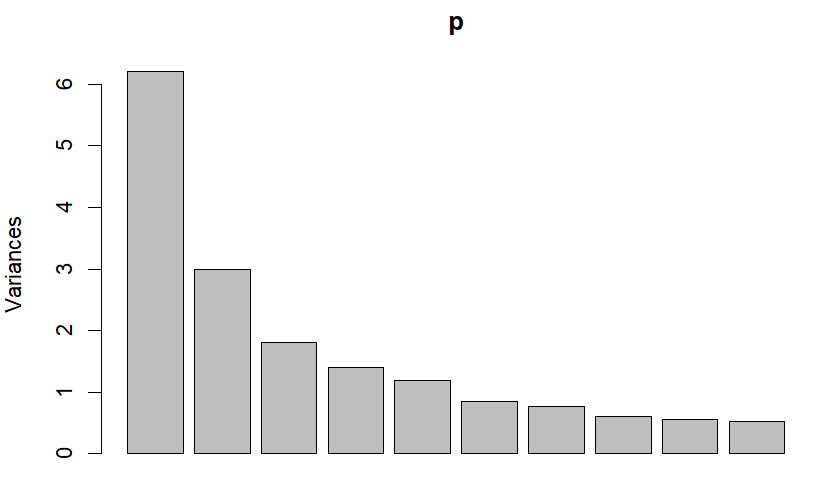
\includegraphics[width=0.8\textwidth]{images/figure_1.png}
    \caption{Scree Plot used to determine CC.}
    \label{fig:figure_1}
\end{figure}

\begin{figure}[h]
    \centering
    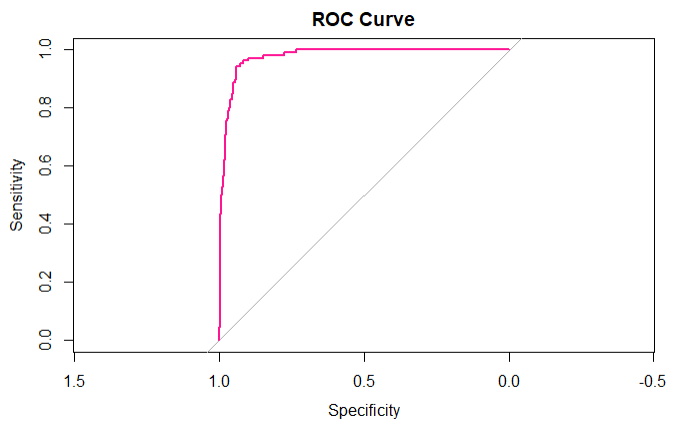
\includegraphics[width=0.8\textwidth]{images/figure_2.png}
    \caption{ROC curve.}
    \label{fig:figure_2}
\end{figure}


\begin{figure}[h]
    \centering
    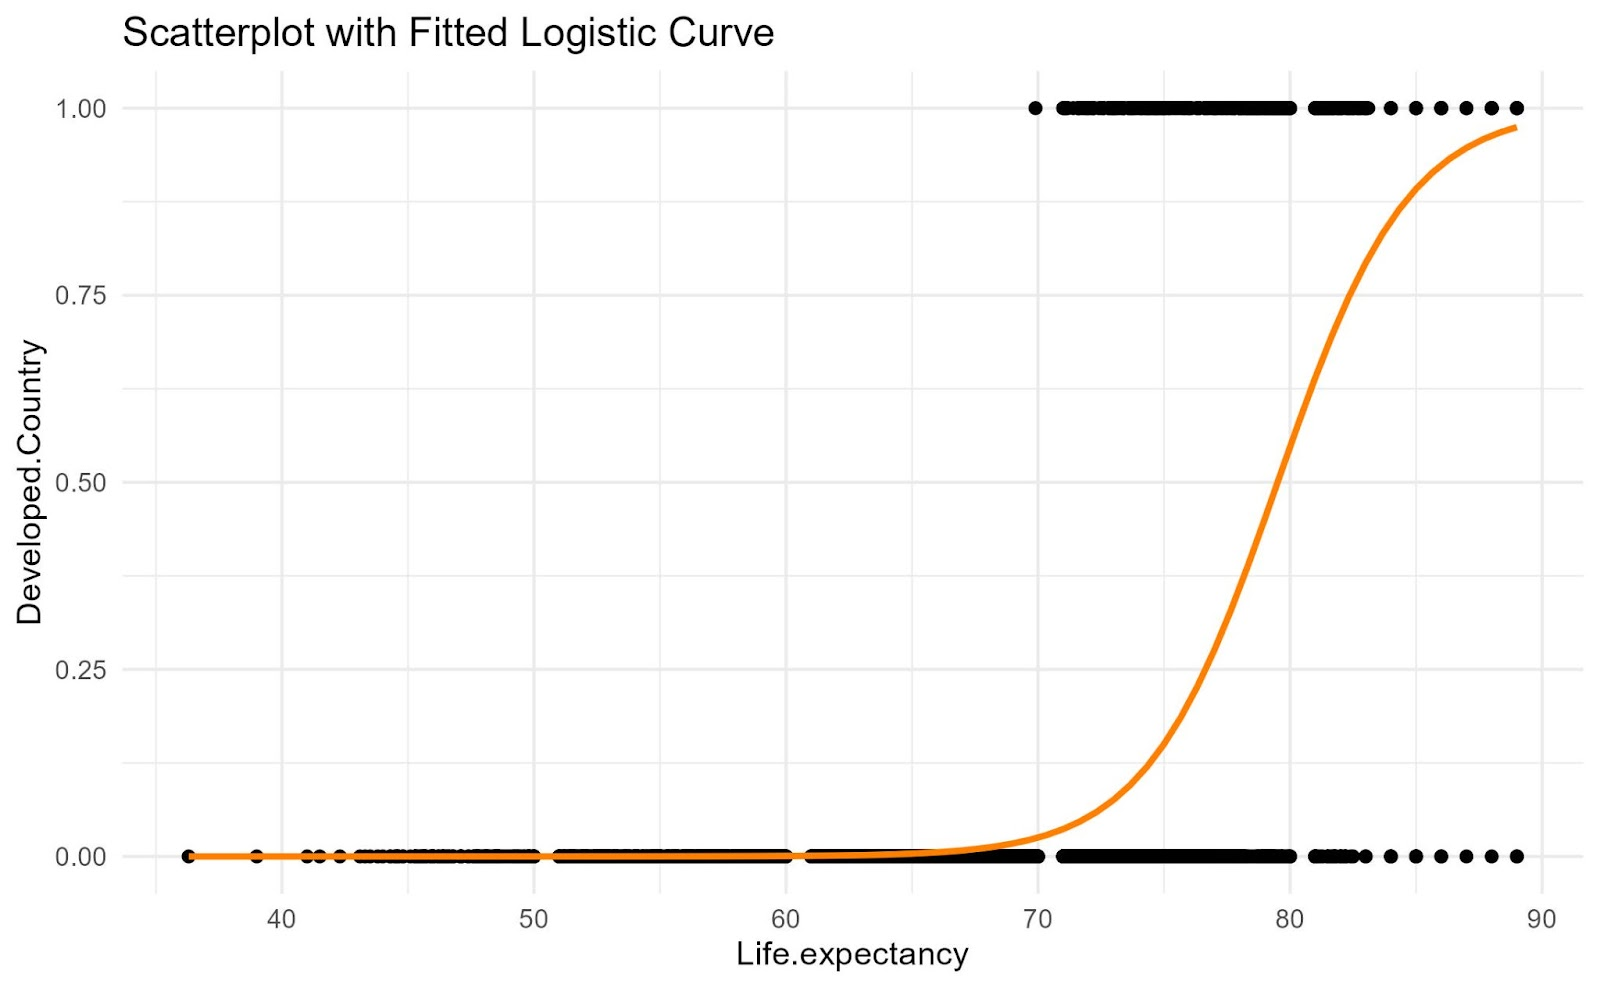
\includegraphics[width=0.8\textwidth]{images/figure_3.png}
    \caption{Adjusted logistic curve.}
    \label{fig:figure_3}
\end{figure}

\begin{figure}[h]
  \centering
  \begin{subfigure}{0.5\textwidth}
    \centering
    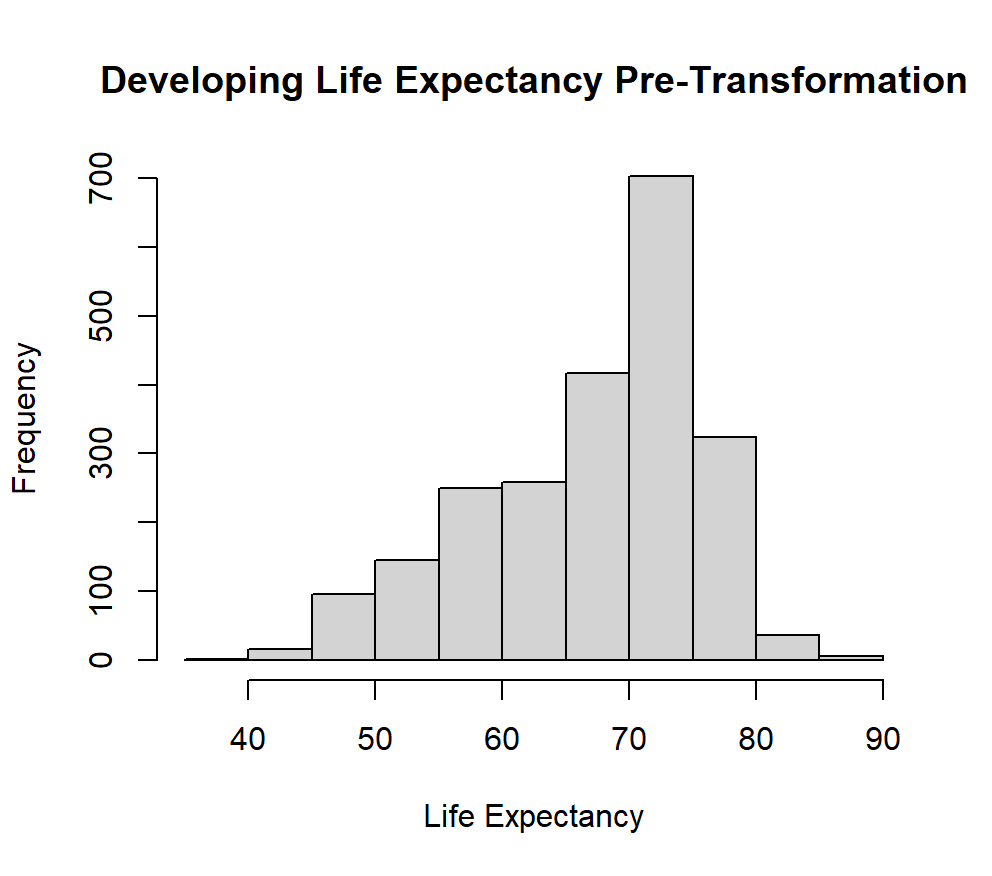
\includegraphics[width=\linewidth]{images/figure_4a.png}
    \caption{Developing: Before}
    \label{subfig:image1}
  \end{subfigure}%
  \begin{subfigure}{0.5\textwidth}
    \centering
    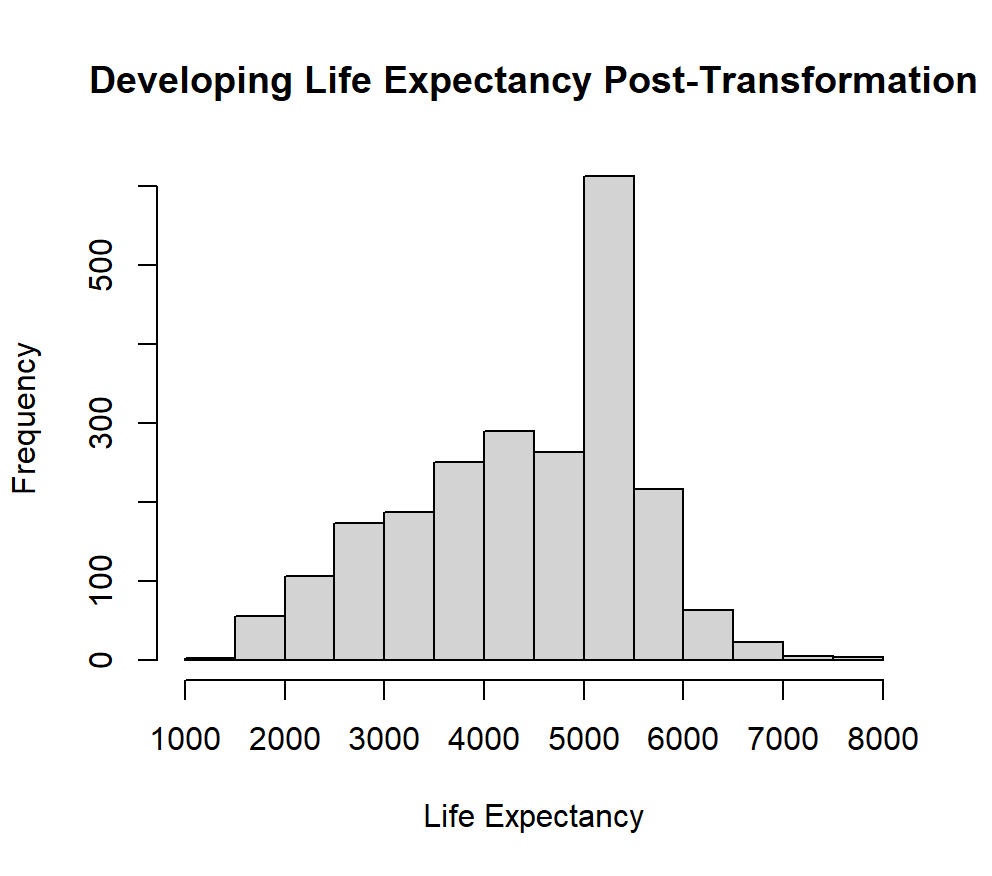
\includegraphics[width=\linewidth]{images/figure_4b.png}
    \caption{Developing: After}
    \label{subfig:image2}
  \end{subfigure}\\[1em]
  \begin{subfigure}{0.5\textwidth}
    \centering
    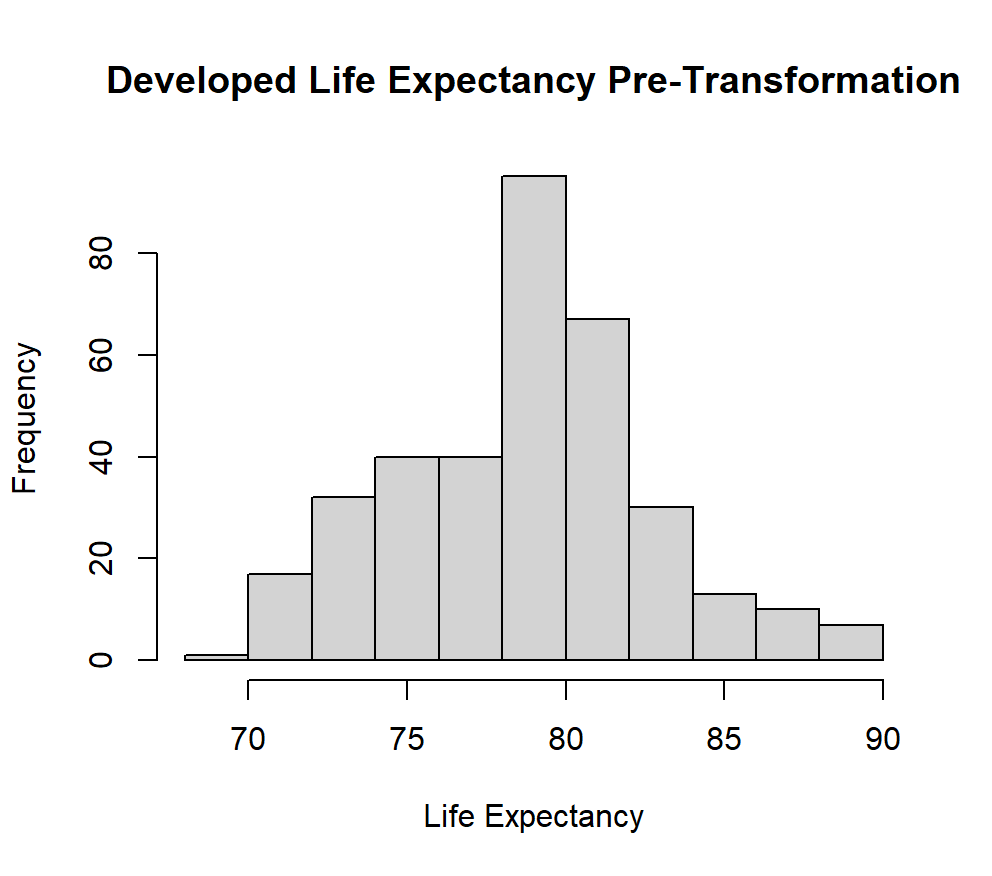
\includegraphics[width=\linewidth]{images/figure_4c.png}
    \caption{Developed: Before}
    \label{subfig:image3}
  \end{subfigure}%
  \begin{subfigure}{0.5\textwidth}
    \centering
    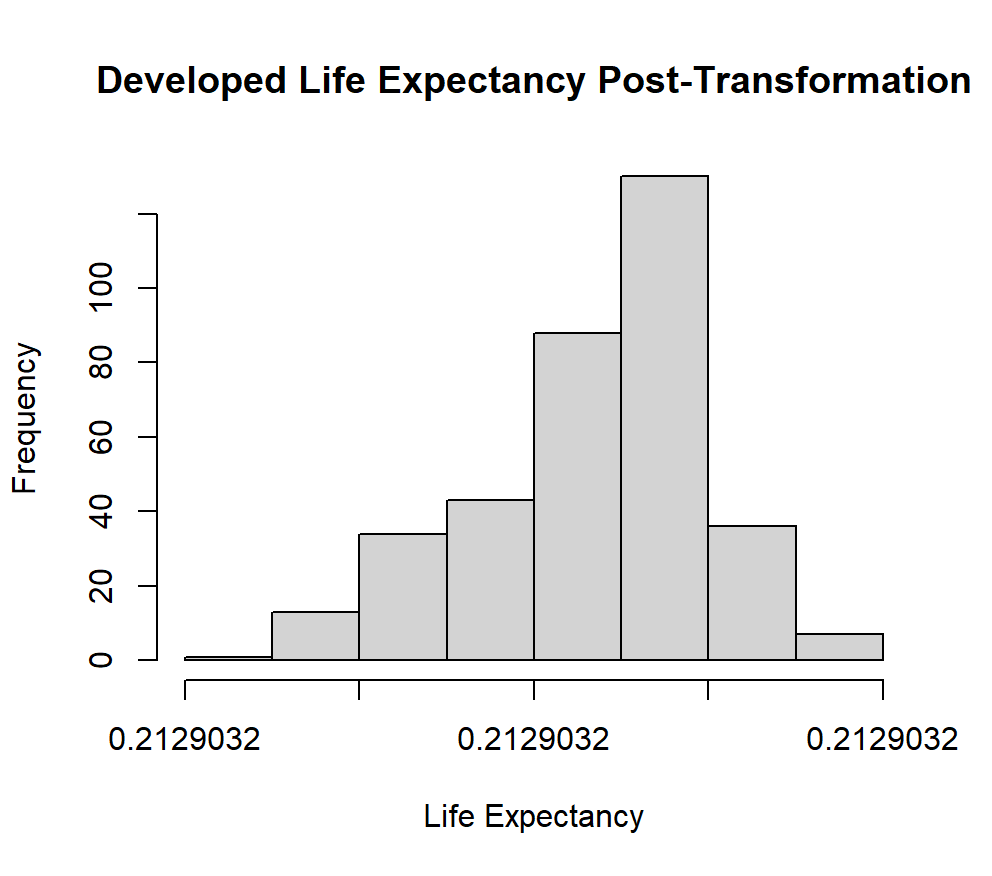
\includegraphics[width=\linewidth]{images/figure_4d.png}
    \caption{Developed: After}
    \label{subfig:image4}
  \end{subfigure}
  \caption{Pre and Post transformed life expectancy for developing and developed countries.}
  \label{fig:figure_4}
\end{figure}

\begin{figure}[h]
    \centering
    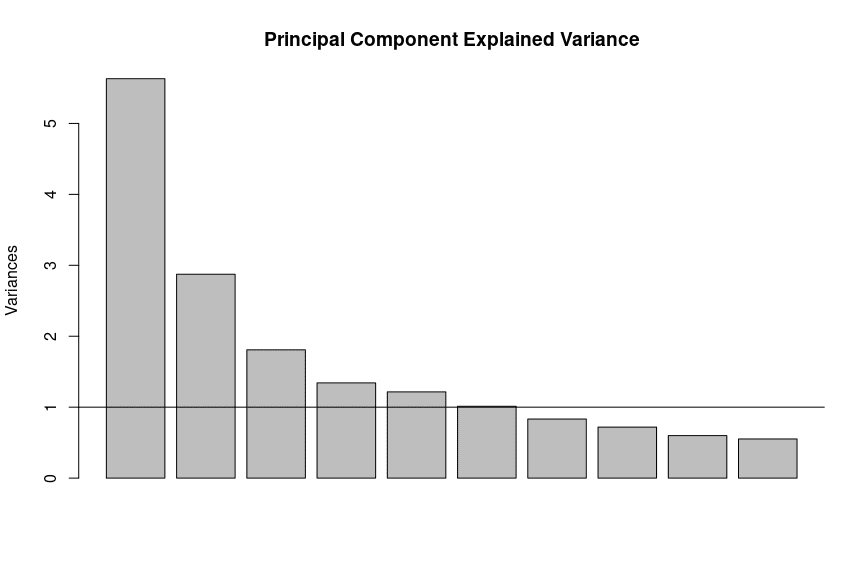
\includegraphics[width=0.8\textwidth]{images/figure_5.png}
    \caption{Cutoff values for principal component analysis.}
    \label{fig:figure_5}
\end{figure}

\begin{figure}[h]
    \centering
    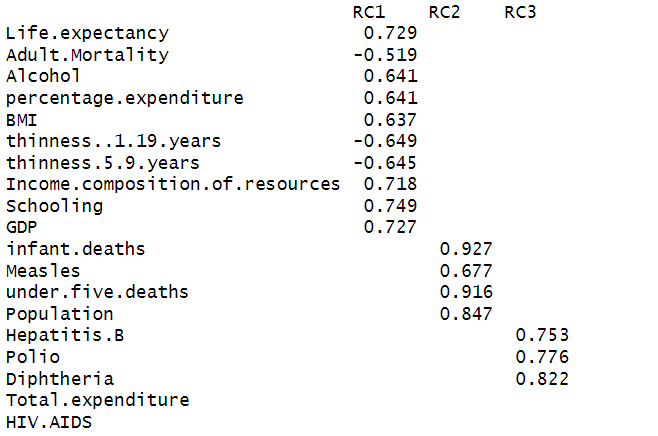
\includegraphics[width=0.7\textwidth]{images/figure_6.png}
    \caption{Results of principal component analysis.}
    \label{fig:figure_6}
\end{figure}

\begin{figure}[h]
    \centering
    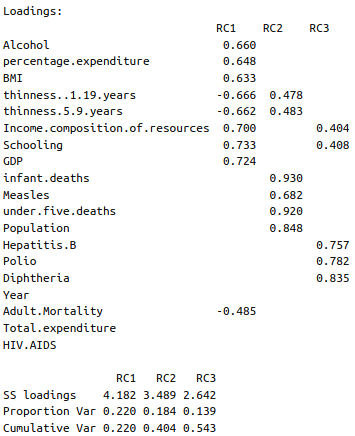
\includegraphics[width=0.6\textwidth]{images/figure_7.png}
    \caption{Factor loadings with a cutoff of 0.4.}
    \label{fig:figure_7}
\end{figure}


\end{document}
